%
% ---------------------------------------------------
%
% Proyecto de Final de Carrera:
% Author: José Lucas Grillo Lorenzo <jlucas.gl@gmail.com>
% Capítulo: Estado del arte en lenguajes de programación paralela 
% Fichero: Cap1_motivation.tex
%
% ----------------------------------------------------
%

\cleardoublepage
\chapter{Modelo poliédrico} \label{chap:polytopes}  

%%% TODO: Escribir introducción.
Desde sus orígenes la informática ha sido fuertemente influenciada por otras ciencias e ingenierías. Es una disciplina en la que confluyen muchas ramas del conocimiento
humano. Destacable es la influencia de las matemáticas, que ha permitido desarrollar 
toda una teoría formal en torno a los lenguajes computables, y eso nos ha permitido definir lo que un artefacto puede hacer y lo que no.

\section{Sobre politopos y la compilación poliédrica}

\subsection{El concepto de politopo en el contexto de los compiladores}


%%%%%%%%%%%%%%%%%%%%%%%%%%%%%%%%%%%%% Figure %%%%%%%%%%%%%%%%%%%%%%%%%%%%%%%%%%%%%%%%%%%%%
\begin{figure}[h]
	\centering
	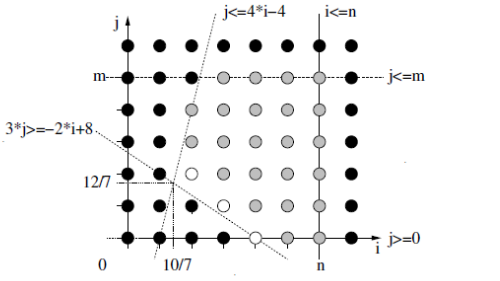
\includegraphics[width=\columnwidth]{poly.png}
	\caption{Representación poliédrica de dos bucles anidados}
	\label{fig:polytope_1}
\end{figure}
%%%%%%%%%%%%%%%%%%%%%%%%%%%%%%%%%%%%%%%%%%%%%%%%%%%%%%%%%%%%%%%%%%%%%%%%%%%%%%%%%%%%%%%%%%

La Matriz \ref{ec:matrix_1} que representa las restricciones de la serie de bucles 
anidados en el Listado \ref{code:polycode1}, delimitará el espacio de iteraciones descrito 
mediante un polígono regular. 
Al tratarse en este caso de un polígono de dos dimensiones se trata de un poliedro, pero 
en general, para espacios de iteraciones $n$-dimensionales, cuando existen $n$ 
bucles anidados, se habla del concepto topológico de politopo.

\subsection{Transformación afín}
